\chapter{Lecture 16: Derivatives of more complicated functions}
In section \ref{derivativetable1} we gave a small table of the derivative formulas that we have come accross. So far, we know how to differentiate some basic functions, and we know how to use linearity to differentiate constant multiples and sums of these functions. \\

\noindent What we do not yet have, is a way to differentiate functions that are products of two or more (non-constant) functions, e.g., $f(x)g(x)$. Nor do we have a way to differentiate functions that are a composition of two or more functions, e.g., $f(g(x))$. We introduced function composition in section \ref{composition (of functions)} (go back and revise if you don't remember). \\

\noindent For example, the function $h(x) = x^3\e^{-x}$ can be viewed as a product of two functions: $f(x) = x^3$ and $g(x) = \e^{-x}$. Also, the function $h(x) = \ln(x^3)$ can be viewed as a composition of $f(x) = \ln(x)$ with $g(x) = x^3$. More examples:
\[
\begin{array}{|c|c|c|c|} \hline
\boldsymbol{h(x)}   	   & \textbf{Type} 		& \boldsymbol{f(x)}  & \boldsymbol{g(x)} \\ \hline
\e^{-\frac{x^2}{2}}  & f(g(x))      			& \e^x			& -\frac{x^2}{2} 	\\ \hline
\e^{-x}			   & f(g(x))				& \e^x 			& -x \\ \hline
-\frac{x^2}{2}		   & f(g(x))				& -\frac{x}{2}		& x^2 \\ \hline
\brac{\sqrt{2}x+17}^6 & f(g(x))			& x^6			& \sqrt{2}x+ 17 \\ \hline
x^7(1-2x)^3		  & f(x)g(x)			& x^7			& (1-2x)^3 \\ \hline		
x^3\ln(x)			  & f(x)g(x)			& x^3			& \ln(x) \\ \hline
x^3 				  & f(x)g(x) 			& x 				& x^2 \\ \hline
\frac{x^2}{\ln(3x)}	 & f(x)g(x)				& x^2			& \frac{1}{\ln(3x)} \\ \hline
\frac{1}{\ln(3x)}	& f(g(x)) 				& x^{-1}			& \ln(3x) \\ \hline
\end{array}
\bigskip
\]
As we can see from the table, the lines are blurry, and functions can often be broken up into compositions or products in more than one way (indeed any function, $h(x)$, is equal to the product of itself with $g(x) = 1$; and is also equal to the composition of itself with $g(x) = x$). The trick, once we have learned the rules for differentiating compositions and products, will be to break the functions up into parts that we know how to differentiate using the formulas that we already have.

\section{Product rule} \label{product rule}
The product rule for differentiating functions of the form $f(x)g(x)$ is

  	\bigskip
	
	\hfil\fbox{
	\begin{minipage}{0.5\columnwidth}{
	
	\vskip 0.02cm
	\begin{center}
	$\displaystyle{\frac{d}{dx}\brac{f(x)g(x)} = f'(x)g(x) + f(x)g'(x)}$
	\end{center}
	}
	\end{minipage}}
	\bigskip

\noindent An alternative way to write this is to let $u = f(x)$ and $v = g(x)$; then

  	\bigskip
	
	\hfil\fbox{
	\begin{minipage}{0.3\columnwidth}{
	
	\vskip 0.02cm
	\begin{center}
	$\displaystyle{\frac{d}{dx}\brac{uv} = u'v + uv'}$
	\end{center}
	}
	\end{minipage}}
	\bigskip

\noindent We will now derive this rule using the definition of a derivative (given in section \ref{rate of change}). Let $f$ and $g$ be real valued functions. We wish to differentiate the function $h(x) = f(x)g(x)$. We have,
\begin{align*}
h'(x) &  = \lim_{h\rightarrow0}\brac{\frac{f(x+h)g(x+h) - f(x)g(x)}{h}} \tag{definition of derivative}
\end{align*}
Now, we have to use a little trick; we will add the expression $f(x+h)g(x) - f(x+h)g(x)$ to the numerator. Notice that this expression is just equal to zero, so adding it does not change the equality. We get,
\begin{align*}
h'(x) &  = \lim_{h\rightarrow0}\brac{\frac{f(x+h)g(x+h) - f(x+h)g(x) + f(x+h)g(x) - f(x)g(x)}{h}} \\
	& =  \lim_{h\rightarrow0}\brac{\frac{f(x+h)\squac{g(x+h) - g(x)} + g(x)\squac{f(x+h) - f(x)}}{h}} \tag{factorising} \\
	& = \lim_{h\rightarrow0}\brac{\frac{f(x+h)\squac{g(x+h) - g(x)}}{h} + \frac{g(x)\squac{f(x+h) - f(x)}}{h}} \tag{fractions} \\
	& =  \lim_{h\rightarrow0}\brac{\frac{f(x+h)\squac{g(x+h) - g(x)}}{h}} + g(x)\lim_{h\rightarrow0}\brac{\frac{f(x+h) - f(x)}{h}}
\end{align*}
The final step was due to the linearity of limits (we can take $g(x)$ outside since it is not dependent on $h$ so it is a constant relative to the limit). Now, the product rule for limits (fact 3, section \ref{limitfacts}) says that the limit of a product is the product of the limits, so we can separate $f(x+h)$ from the rest to get
\[
h'(x) = \lim_{h\rightarrow0}\brac{f(x+h)}\lim_{h\rightarrow0}\brac{\frac{g(x+h) - g(x)}{h}} + g(x)\lim_{h\rightarrow0}\brac{\frac{f(x+h) - f(x)}{h}}
\]
As $h \rightarrow 0$, $f(x + h) \rightarrow f(x)$, so we can simplify this to
\[
h'(x) = f(x)\lim_{h\rightarrow0}\brac{\frac{g(x+h) - g(x)}{h}} + g(x)\lim_{h\rightarrow0}\brac{\frac{f(x+h) - f(x)}{h}}
\]
Notice that this expression contains the definitions of the derivatives $g'(x)$ and $f'(x)$, meaning that
\[
h'(x) = f(x)g'(x) + g(x)f'(x).
\] 
Which is the product rule, as required.

\subsection{Example}
Differentiate $x^7\ln(x^3)$ \\

\solution
Let $h(x)= x^7\ln(x^3)$. Then $h(x) = f(x)g(x)$, where $f(x) = x^7$ and $g(x) = \ln(x^3)$. We can use the log laws to simplify the latter, giving 
\[
g(x) = \ln(x^3) = 3\ln(x) \tag{logarithm laws}
\]
Now,
\[
f'(x) = 7x^6 \qquad \text{and} \qquad g'(x) = \frac{3}{x} \tag{using derivative formulas}
\]
We now have $f(x),g(x),f'(x)$, and $g'(x)$, which is enough to use the product rule. The product rule says that
\begin{align*}
h'(x) & = f'(x)g(x) + f(x)g'(x) \\
	& = 7x^63\ln(x) + x^7 \frac{3}{x} \tag{plugging in our results} \\
	& = 21x^6\ln(x) + 3x^6 \\
	& = 3x^6(7\ln(x) + 1). \tag{factorising}
\end{align*}

\section{Chain rule} \label{chain rule}
The chain rule, for differentiating functions of the form $f(g(x))$ (a composition of functions) is

  	\bigskip
	
	\hfil\fbox{
	\begin{minipage}{0.4\columnwidth}{
	
	\vskip 0.02cm
	\begin{center}
	$\displaystyle{\frac{d}{dx}\brac{f(g(x))} = f'(g(x))g'(x)}$
	\end{center}
	}
	\end{minipage}}
	\bigskip
	
\noindent This means that first we differentiate $f(g(x))$, with respect to $g(x)$ (so we treat $g(x)$ as if it were the variable, e.g., $x$), then we differentiate $g(x)$ with respect to $x$ (and multiply the results). We can rewrite this in different notation, as follows: Let $u = g(x)$. Then $f(g(x)) = f(u)$. The chain rule is:
\[
\frac{d}{dx}\brac{f(u)} = f'(u)u'(x)
\]
Replacing $g(x)$ with $u$ helps us illustrate that we are differentiating with respect to $g(x)$ (i.e., $u$) in the first step, rather than $x$. It might seem strange to replace a function, $g(x)$, with a variable, $u$, but $u$ is still a function (it still makes sense to write $u(x)$). \\
Sometimes, you might see the chain rule written:
\[
\frac{d}{dx}\brac{f(u)} = \frac{d}{du}\brac{f(u)}\frac{d}{dx}\brac{u(x)}
\]
Or even
\[
\frac{d}{dx}\brac{f(u)} = \frac{df}{du}\frac{du}{dx} \tag{where $u = g(x)$}
\]
Which both mean the same thing. \\

\noindent We will now derive the chain rule using the definition of a derivative. We wish to differentiate the function $h(x) = f(g(x))$. We have
\begin{align*}
h'(x)& = \lim_{h \rightarrow 0}\brac{\frac{f(g(x+h)) - f(g(x))}{h}} \tag{definition of a derivative}
\end{align*}
Now, we will multiply the expression inside the limit by $\frac{g(x+h) - g(x)}{g(x+h) - g(x)}$. Notice that this is just equal to 1, so we are not changing the equality. We get,
\begin{align*}
h'(x) & = \lim_{h \rightarrow 0}\brac{\frac{f(g(x+h)) - f(g(x))}{g(x+h) - g(x)}\frac{g(x+h) - g(x)}{h}}  \\
	& =  \lim_{h \rightarrow 0}\brac{\frac{f(g(x+h)) - f(g(x))}{g(x+h) - g(x)}}\lim_{h \rightarrow 0}\brac{\frac{g(x+h) - g(x)}{h}} \\
	& = f'(g(x))g'(x). \tag{definition of a derivative}
\end{align*}
In the second last step we used the product rule for limits. Now, this derivation was not entirely sound. The expression obtained in the second last step might not be defined, and may result in division by zero, given certain conditions. Unfortunately, a perfectly accurate proof is slightly outside the scope of this course. \\ 

%Let $f(u) = \e^u$ and let $u = ax$. Then $h(x) = f(u)$. Now,
%\[
%f'(u) = \frac{d}{dx}\brac{\e^x} = \e^x \qquad \text{and} \qquad u'(x) = \frac{d}{dx}\brac{ax} = a  \tag{derivative formulas}
%\]
%By the chain rule:
%\begin{align*}
%h'(x) & = f'(u)u'(x) \\
%	& = \e^xa.
%\end{align*}

\subsection{Example}
Differentiate $\e^{-\frac{x^2}{2}}$.  \\

\solution
Let $h(x) = \e^{-\frac{x^2}{2}}$. Let $f(u) = \e^u$ and let $u = -\frac{x^2}{2}$. Then $h(x) = f(u)$. We have
\[
f'(u) = \e^u \qquad \text{and} \qquad u'(x) = \frac{d}{dx}\brac{-\frac{x^2}{2}} = -x \tag{derivative formulas}
\]
By the chain rule:
\begin{align*}
h'(x) & = f'(u)u'(x) \\
	& = \e^u\times(-x) \tag{plugging in our results} \\
	& = -x\e^{-\frac{x^2}{2}}. \tag{since $u = -\frac{x^2}{2}$}
\end{align*}

\subsection{Example}
Differentiate $\ln(x^4 + 2x^2)$ \\

\solution
Let $h(x) = \ln(x^4 + 2x^2)$. Let $f(u) = \ln(u)$ and let $u = x^4 + 2x^2$. Then $h(x) = f(u)$. We have
\[
f'(u) = \frac{1}{u} \qquad \text{and} \qquad u'(x) = 4x^3 + 4x = 4(x^3 + x)
\]
By the chain rule:
\begin{align*}
h'(x) & = f'(u)u'(x) \\
	& = \frac{1}{u}\times4(x^3 + x) \tag{plugging in our results} \\
	& = \frac{4x^3 + x}{x^4 + 2x^2} \tag{since $u = x^4 + 2x^2$} \\
	& = \frac{4x^2 + 1}{x^3 + 2x}. \tag{cancelling common factor, $x$}
\end{align*}

\subsection{Example} \label{ex16.1}
\noindent When we found the derivative of the exponential function, $\frac{d}{dx}\brac{\e^{x}} = \e^x$, in section \ref{derivative of exponential}, we also gave a more general rule,
\[
\frac{d}{dx}\brac{ \e^{ax}} = a\e^{ax}.
\]
At the time, we mentioned that this fact will be more obvious once we learn the chain rule. This is because we can derive it using the formulas for the derivative of $\e^x$, and that of $ax$. \\

\noindent We will go one small step further here; we wish to differentiate $h(x) = \e^{ax+b}$. Let $u = ax+b$.
By the chain rule, we have
\begin{align*}
\frac{d}{dx}\brac{\e^{ax+b}} & = \frac{d}{du}\brac{\e^{u}}\frac{d}{dx}\brac{ax+b} \\
					     & = \e^ua \tag{derivative formulas} \\
					     & = a\e^{ax+b}. \tag{since $u = ax+b$}
\end{align*}

\subsection{The simplest type of chain} \label{simplest chain}
In example \ref{ex16.1}, using the chain rule was very straight forward. This was partly because the function $h(x) = \e^{ax}$ has a particular structure; it is of the form 
\[
h(x) = f(ax + b) \tag{where $f(x) = \e^x$}
\]
We can write $h(x) = f(u)$, with $u = ax + b$. So,
\[
u'(x) = \frac{d}{dx}\brac{ax+b} = \frac{d}{dx}\brac{ax} + \frac{d}{dx}\brac{b} = a \tag{linearity, and derivative formulas}
\]
Hence, by the chain rule
\[
h'(x) = f'(u)u'(x) = f'(u)a
\]
Since $u = ax+b$ we get $h'(x) = f'(ax+b)a$. \textbf{So, we have derived a simple formula:}

  	\bigskip
	
	\hfil\fbox{
	\begin{minipage}{0.6\columnwidth}{
	
	\vskip 0.02cm
	\begin{center}
	$\displaystyle{h(x) = f(ax+b) \;\;\; \text{implies} \;\;\; h'(x) = af'(ax+b)}$
	\end{center}
	}
	\end{minipage}}
	\bigskip
	
\subsection{Example}
We do not necessarily need to commit to memory the formula in section \ref{simplest chain}; it is perfectly good practice to use the chain rule every time (it will probably help you become efficient with the chain rule if you use it every time). However, the formula may make our job easier and quicker. \\

\noindent \textbf{Example 1:} \\
\noindent Differentiate $(2x+17)^8$ \\

\solution
Notice that $2x+17$ has the form $ax+b$, with $a = 2$ (and $b = 17$).  \\

%Let $h(x) = (2x+17)^8$. Let $f(u) = u^8$ with $u = 2x+ 17$. Then 
%\[
%f'(u) = 8u^7 = 8(2x+17)^7
%\] 
%Using the formula in section \ref{simplest chain} we have
%\[
%h'(x) = af'(ax+b) = 2\times f'(2x+17) = 2\times8(2x+17)^7 = 16(2x+17)^7
%\]
\noindent Let $h(x) = (2x+17)^8$. Then $h(x) = f(2x+17)$ where $f(x) = x^8$. Hence, using the formula in section \ref{simplest chain} we have
\[
h'(x) = 2\times f'(2x+17) = 2\times8(2x+17)^7 = 16(2x+17)^7.
\]

\noindent \textbf{Example 2:} \\
\noindent Differentiate $\e^{7-x}$. \\

\solution
Notice that $7-x$ has the form $ax+b$ with $a = -1$ (and $b = 7$). \\

\noindent Let $h(x) = \e^{7-x}$. Then $h(x) = f(7-x)$ with $f(x) = \e^x$. Hence, using the formula in section \ref{simplest chain} we have
\[
h'(x) = -1\times f'(7-x) = -\e^{7-x}.
\]
This is quicker than the way we differentiated $\e^{7-x}$ in example \ref{ex12.101}.

\section{Products involving chains}
Let's break $x^7(1-x)^3$ into a product of two functions: Let $f(x) = x^7$ and let $g(x) = (1-x)^3$. We can easily find $f'(x) = 7x^6$. However, we do not have a simple formula for differentiating $g(x) = (1-x)^3$. \\

\noindent Thankfully, $g(x)$ is a composition of two functions that we do know how to differentiate. Conveniently, $g(x)$ even has the form of a simple chain as described in section \ref{simplest chain}. \\

\noindent We have $g(x) = k(1-x)$, with $k(x) = x^3$. Hence, using the formula for simple chains,
\[
g'(x) = -1\times k'(1-x) = -1\times3(1-x)^2 = -3(1-x)^2.
\]
So far we have found that
\[
f(x) = x^7, \;\;\; f'(x) = 7x^6, \;\;\; g(x) = (1-x)^3 \;\; \text{and} \;\; g'(x) = -3(1-x)^2.
\]
We can now use the product rule to find $f(x)g(x)$. Using the product rule:
\begin{align*}
\frac{d}{dx}\brac{x^7(1-x)^3} & = f'(x)g(x) + f(x)g'(x) \\
		& = 7x^6 \times(1-x)^3 + x^7\times(-3(1-x)^2) \tag{plugging in our results} \\
		& = 7x^6(1-x)^3 - 3x^7(1-x)^2.
\end{align*}
This could be simplified further, but we will stop here since we have achieved what we wanted.

\subsection{Example} \label{ex16.4}
Suppose that we wish to differentiate $h(x) = \frac{x^2}{\ln(x)}$. We could treat this as a product, breaking it up into $f(x) = x^2$ and $g(x) = \frac{1}{\ln(x)}$. We can immediately find $f'(x) = 2x$. However, we do not have a simple formula for differentiating $\frac{1}{\ln(x)}$. \\

\noindent The problem is resolved when we realise that $g(x) = \frac{1}{\ln(x)}$ is a composition of two functions: Let $k(u) = u^{-1}$ and let $u = \ln(x)$. Then $g(x) = k(u)$. It follows that
\[
k'(u) = -u^{-2} \qquad \text{and} \qquad u'(x) = \frac{1}{x}. \tag{derivative formulas}
\]
Hence, using the chain rule:
\begin{align*}
g'(x) & = k'(u)u'(x) \\
	& = -u^{-2}\times\frac{1}{x} \tag{derivative formulas} \\
	& = -\frac{(\ln(x))^{-2}}{x} \tag{since $u = \ln(x)$} \\
	& = -\frac{1}{x(\ln(x))^2}. \tag{index laws}
\end{align*}
Now we have $f'(x),g'(x),f(x)$ and $g(x)$, which is enough to use the product rule. Using the product rule:
\begin{align*}
h'(x) & = f'(x)g(x) + f(x)g'(x) \\
	& = 2x\times\frac{1}{\ln(x)} + x^2\times\brac{-\frac{1}{x(\ln(x))^2}} \tag{plugging in our results} \\
	& = \frac{2x}{\ln(x)} - \frac{x}{(\ln(x))^2}. \tag{simplifying}
\end{align*}
We could certainly simplify this expression further, but we have achieved what we set out to do; simplifying is left as an exercise to the reader.

\section{The quotient rule} \label{quotient rule}
Here we will introduce a new rule, which is used to differentiate functions of the form $h(x) = \frac{f(x)}{g(x)}$; functions like these are called \textbf{quotient functions} (or sometimes called \textbf{rational functions}). \\ 

\noindent \textbf{The quotient rule is:}

  	\bigskip
	
	\hfil\fbox{
	\begin{minipage}{0.55\columnwidth}{
	
	\vskip 0.02cm
	\begin{center}
	$\displaystyle{\frac{d}{dx}\brac{\frac{f(x)}{g(x)}} = \frac{f'(x)g(x) - f(x)g'(x)}{g(x)^2}}$
	\end{center}
	}
	\end{minipage}}
	\bigskip
	


\noindent In the previous example (example \ref{ex16.4}), we differentiated $h(x) = \frac{x^2}{\ln(x)}$ (a quotient function) using only the chain rule and product rule. It is perfectly reasonable to use the chain rule and product rule every time you differentiate a quotient function. The quotient rule is really just a faster formula to complete the same process; it is derived entirely from the chain rule and the product rule, as follows: \\

\noindent Let $h(x) = \frac{f(x)}{g(x)}$. Then
\begin{align*}
h(x) & = f(x)g(x)^{-1} \tag{index laws} \\
	& = f(x)k(x), \;\;\; \text{where we let $k(x) = g(x)^{-1}$}
\end{align*}
The derivative of $k(x)$ is given by the chain rule. Let $g(x) = u$. Then $k(u) = u^{-1}$. So,
\[
k'(u) = -u^{-2} \qquad \text{and} \qquad u'(x) = g'(x). \tag{derivative formulas}
\]
So, by the chain rule we have
\begin{align*}
k'(x) & = k'(u)u'(x) \\
	& = -u^{-2}g'(x) \tag{plugging in our results} \\
	& = -g(x)^{-2}g'(x). \tag{since $u = g(x)$} \\
	& = -\frac{g'(x)}{g(x)^2}. \tag{index laws}
\end{align*}
We can now use the product rule to find $h'(x)$. We get
\begin{align*}
h'(x) & = f'(x)k(x) + f(x)k'(x) \\
	& = f'(x)g(x)^{-1} + f(x)\times\brac{-\frac{g'(x)}{g(x)^2}} \tag{plugging in our results} \\
	& = \frac{f'(x)g(x)}{g(x)^2} - \frac{f(x)g'(x)}{g(x)^2} \tag{multiplying first term by $\frac{g(x)}{g(x)} = 1$} \\
	& = \frac{f'(x)g(x) - f(x)g'(x)}{g(x)^2}. \tag{combining fractions}
\end{align*}
Which is the quotient rule, as required.

\subsection{Example}
Differentiate $\frac{\e^{3x+12}}{\ln(3x)}$. \\

\solution
Let $h(x) = \frac{\e^{3x+12}}{\ln(3x)}$. Let $f(x) = \e^{3x+12}$ and let $g(x) = \ln(3x)$. Then $h(x) = \frac{f(x)}{g(x)}$. Now
\[
f'(x) = 3\e^{3x+12} \;\;\; \text{and} \;\;\; g'(x) = 3\frac{1}{3x} = \frac{1}{x}. \tag{simple chains (section \ref{simplest chain})}
\]
Using the chain rule:
\begin{align*}
h'(x) 		& = \frac{f'(x)g(x) - f(x)g'(x)}{g(x)^2} \\
		& = \frac{3\e^{3x+12}\ln(3x) - \e^{3x+12}\frac{1}{x}}{(\ln(3x))^2} \tag{plugging in our results} \\
		& = \frac{3\e^{3x+12}}{(\ln(3x))^2}\brac{\ln(3x) - \frac{1}{x}}. \tag{factorising}
\end{align*}

\section{Definition of mode (and how to find it)} \label{mode definition}
\noindent In example \ref{mode1(notreally)}, and in section \ref{check poi(lambda)}, we used the term, ``mode,'' which we defined to be whichever output of the random variable that has the highest probability associated with it (i.e., the most probable outcome). \\

\noindent In section \ref{turning points}, we learned how to use calculus to find stationary points of continuous functions (go back and revise this now if you don't remember). We also mentioned that,  for continuous distributions, a particular kind of stationary point, called a global maximum, corresponds to the \textbf{mode} (since a global maximum is the highest point obtained by a function). \\


\noindent More accurately, for a continuous distribution with probability density function, $f$,

  	\bigskip
	
	\hfil\fbox{
	\begin{minipage}{0.55\columnwidth}{
	
	\vskip 0.02cm
	\begin{center}
	The \textbf{mode} is the input value, $x$, such that $f(x)$ is a global maximum. At any stationary point we have $f'(x) = 0.$
	\end{center}
	}
	\end{minipage}}
	\bigskip
	
\noindent Recall from section \ref{turning points} that, for a function $f$, a stationary point is defined to be a point where $f'(x) = 0$. A global maximum is a type of stationary point. In the following example, we will see how to use this fact to find the mode.

\subsection{Example}
In section \ref{cdf(continuous)}, we mentioned that the pdf of a continuous distribution can be obtained from its cdf by differentiation (since the cdf is an antiderivative of the pdf). \\

\noindent For the following function
\[
F(x) = \left\{ \begin{array}{ll}
0, & \; \text{if} \; x < 0 \smallskip \\
1 - \exp(-x^2), & \; \text{if} \; x \geq 0
\end{array} \right.
\]
Check that $F$ has the typical features of a cdf (see section \ref{cdf(continuous)}). Find the associated pdf, $f(x)$. Then find the mode. \\

\solution
The output values of a cdf should all lie in the set $[0,1]$ and be non-decreasing; also, as $x \rightarrow \infty$ we require $F(x) \rightarrow 1$, and as $x \rightarrow -\infty, F(x) \rightarrow 0$. We will sketch a graph of $F$ to check that these conditions hold. Then we will use differentiation to find the pdf and the mode. \\

\noindent \textbf{Sketch the graph} \\
\noindent We know from section \ref{bell curve}, that $\exp(-x^2)$ is a Gaussian (i.e., a bell curve), of height $1$, centered at the origin. So, $-\exp(-x^2)$ (taking the negative) gives an upside down bell curve (i.e., flipped accross the $x$-axis), as in Graph $A$ below. \\

\noindent Adding $1$ to this (to give $1 - \exp(-x^2))$ increases the output value by 1 everywhere; so, it moves the whole graph up the $y$-axis by a distance of $1$. This is called a \textbf{translation} up the $y$-axis (by 1). This gives Graph $B$ below. \label{translation(sort of)}
\begin{center}
\begin{minipage}{0.4\textwidth}
	\begin{center}
	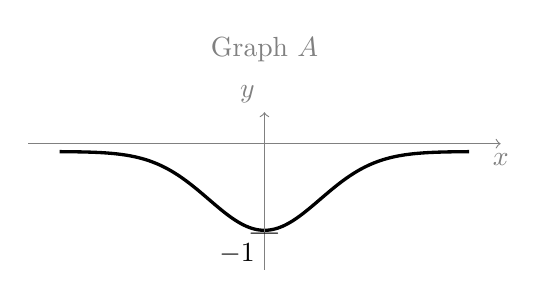
\begin{tikzpicture}
	\draw [gray] (0,1.3) node {Graph $A$};
	\draw [very thick] plot [samples = 200, domain = -2.6:2.6, smooth] (\x,{-exp(-\x*\x)});
	\draw [->,gray] (-3,0.1) -- (3,0.1) node [below] {$x$};
	\draw [->,gray] (0,-1.5) -- (0,0.5) node [above left] {$y$};
	\draw (0,-1.04) node [rotate = 90] {$|$} node [below left] {$-1$}; 
	\end{tikzpicture}
	\end{center}
\end{minipage}
\begin{minipage}{0.1\textwidth}
\begin{center}
	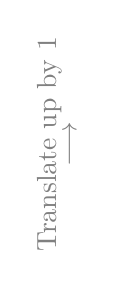
\begin{tikzpicture}
	\draw [gray] (0,0) node [rotate = 90] {$\longrightarrow$} node [rotate = 90, above] {Translate up by $1$};
	\end{tikzpicture}
\end{center}
\end{minipage}
\begin{minipage}{0.4\textwidth}
	\begin{center}
	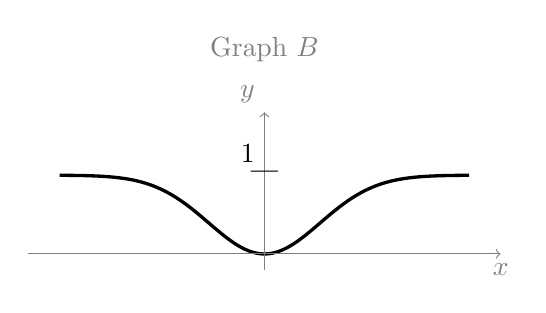
\begin{tikzpicture}
	\draw [gray] (0,2.6) node {Graph $B$};
	\draw [very thick] plot [samples = 200, domain = -2.6:2.6, smooth] (\x,{1-exp(-\x*\x)});
	\draw [->,gray] (-3,0) -- (3,0) node [below] {$x$};
	\draw [->,gray] (0,-0.2) -- (0,1.8) node [above left] {$y$};
	\draw (0,1.04) node [rotate = 90] {$|$} node [above left] {$1$}; 
	\end{tikzpicture}
	\end{center}
\end{minipage}
\end{center}
Now, $F(x) = 1-\exp(-x^2)$ when $x \geq 0$ and $F(x) = 0$ otherwise. Hence the graph of $F(x)$ looks like:
\begin{center}
	\begin{tikzpicture}
	\draw [very thick] (-1,0) -- (0,0); 
	\draw [very thick] plot [samples = 200, domain = 0:2.6, smooth] (\x,{1-exp(-\x*\x)});
	\draw [->,gray] (-1,0) -- (3,0) node [below] {$x$};
	\draw [->,gray] (0,-0.2) -- (0,1.8) node [above left] {$y$};
	\draw (0,1.04) node [rotate = 90] {$|$} node [above left] {$1$};
	\end{tikzpicture}
\end{center}
We can see that the output values all lie between 0 and 1, and that the output increases from 0 to 1, as required. \\

\noindent \textbf{Find the pdf} \\
Since $F(x)$ is an antiderivative of $f(x)$ we have $F'(x) = f(x)$. For $x < 0$, $F(x) = 0$, so $F'(x) = 0$. For $x \geq 0$ we have
\begin{align*}
F'(x) & = \frac{d}{dx}\brac{1 - \exp(-x^2)}  \\
	& = - \frac{d}{dx}\brac{\exp(-x^2)} \tag{since $\frac{d}{dx}(1) = 0$} \\
	& = -\frac{d}{dx}\brac{-x^2}\exp(-x^2)  \tag{chain rule, and $\frac{d}{dx}\brac{\e^x} = \e^x$} \\
	& = 2x\exp(-x^2) \tag{a derivative formula}
\end{align*}
Putting these together we get the pdf:
\[
	f(x) = \left\{
	\begin{array}{ll}
	0, & \; \text{if} \; x < 0 \smallskip \\
	2x\exp(-x^2), & \; \text{if} \; x \geq 0
	\end{array}
	\right.
\]

\noindent \textbf{Find the mode} \\
The mode of the distribution will be somewhere where $f(x)$ is non-zero. So, we need only concern ourselves with the domain $x \geq 0$, where $f(x) = 2x\exp(-x^2)$. \\

\noindent The mode is a stationary point, so we must have $f'(x) = 0$ at the mode. To differentiate $f(x)$ we need the product rule. Let $k(x) = 2x$ and let $g(x) = \exp(-x^2)$. Then $f(x) = k(x)g(x)$ and
\[
k'(x) = 2 \;\;\; \text{and} \;\;\; g'(x) = \frac{d}{dx}\brac{-x^2}\exp(-x^2) = -2x\exp(-x^2) \tag{chain rule}
\]
By the product rule:
\begin{align*}
f'(x)  & = k'(x)g(x) + k(x)g'(x) \\
	& = 2\times\exp(-x^2) + 2x\times\brac{-2x\exp(-x^2)} \tag{plugging in our results} \\
	& = 2\exp(-x^2) -4x^2\exp(-x^2) \\
	& = 2\exp(-x^2)\brac{1 - 2x^2} \tag{factorising}
\end{align*}
Now, we are looking for $x$ such that $f'(x) = 0$. So we need to solve for $x$ in the following equation
\[
2\exp(-x^2)\brac{1-2x^2} = 0.
\]
The term $\exp(-x^2)$ can never be equal to zero (see section \ref{exponentials}). So we require
\[
1-2x^2 = 0, \qquad \text{which is true if} \qquad x = \frac{1}{\sqrt{2}} \tag{solving for $x$}
\]
Notice that we have a positive square root, since we are only concerned with $x \geq 0$. Remember, stationary points are not necessarily always maxima (they could otherwise be minima or points of inflection), but the following line of reasoning is sufficient to conclude that $x = \frac{1}{\sqrt{2}}$ is a maximum: \\

As $x = \frac{1}{\sqrt{2}}$ is the only value that gives $f'(x) = 0$ (i.e., the only value that gives a stationary point), and since we know that there exists a maximum, we conclude that $x = \frac{1}{\sqrt{2}}$ is the maximum. \\

\noindent In other instances, you might end up finding two or more possible values of $x$ that correspond to stationary points. In such a situation, you need to use other information available to you to decide which value of $x$ must be the maximum. For example, you might know that $x > 0$.